\documentclass[tikz,border=6pt]{standalone}
\usepackage{lmodern}
\usepackage{amsmath}
\usetikzlibrary{calc}
\definecolor{ablue}{RGB}{38,84,160}
\definecolor{sorange}{RGB}{214,110,22}
\definecolor{plane}{RGB}{232,235,241}
\begin{document}
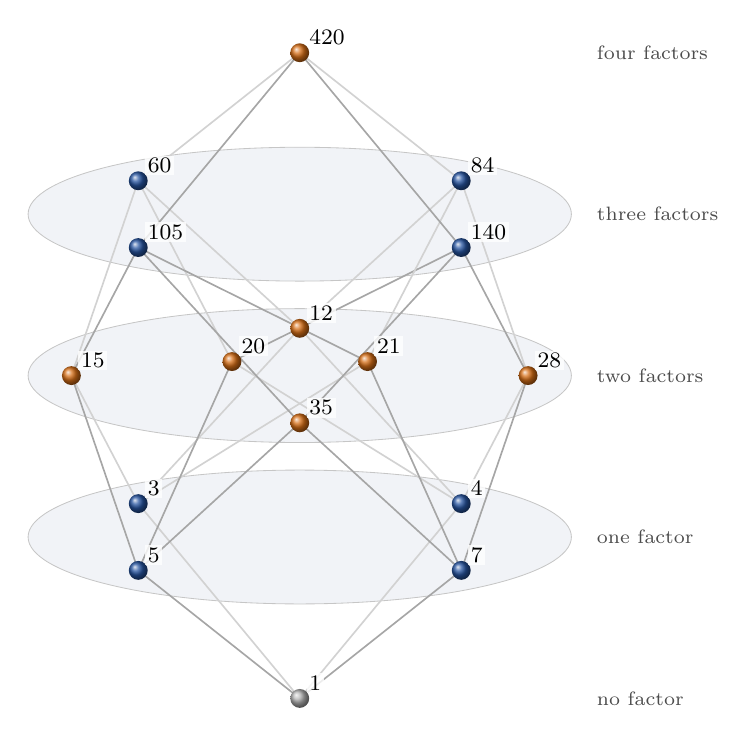
\begin{tikzpicture}
\fill[plane,opacity=0.6] (0,2.050) ellipse[x radius=3.45,y radius=0.85];
\draw[gray!45,line width=0.3pt] (0,2.050) ellipse[x radius=3.45,y radius=0.85];
\node[font=\scriptsize,gray!60!black,anchor=west] at (3.65,2.050) {one factor};
\fill[plane,opacity=0.6] (0,4.100) ellipse[x radius=3.45,y radius=0.85];
\draw[gray!45,line width=0.3pt] (0,4.100) ellipse[x radius=3.45,y radius=0.85];
\node[font=\scriptsize,gray!60!black,anchor=west] at (3.65,4.100) {two factors};
\fill[plane,opacity=0.6] (0,6.150) ellipse[x radius=3.45,y radius=0.85];
\draw[gray!45,line width=0.3pt] (0,6.150) ellipse[x radius=3.45,y radius=0.85];
\node[font=\scriptsize,gray!60!black,anchor=west] at (3.65,6.150) {three factors};
\node[font=\scriptsize,gray!60!black,anchor=west] at (3.65,8.200) {four factors};
\node[font=\scriptsize,gray!60!black,anchor=west] at (3.65,0.000) {no factor};
\draw[gray!35,line width=0.6pt] (0.000,0.000) -- (2.051,2.474);
\draw[gray!35,line width=0.6pt] (0.000,0.000) -- (-2.051,2.474);
\draw[gray!70,line width=0.6pt] (0.000,0.000) -- (-2.051,1.626);
\draw[gray!70,line width=0.6pt] (0.000,0.000) -- (2.051,1.626);
\draw[gray!35,line width=0.6pt] (2.051,2.474) -- (0.000,4.700);
\draw[gray!35,line width=0.6pt] (2.051,2.474) -- (-0.861,4.278);
\draw[gray!35,line width=0.6pt] (2.051,2.474) -- (2.900,4.100);
\draw[gray!35,line width=0.6pt] (-2.051,2.474) -- (0.000,4.700);
\draw[gray!35,line width=0.6pt] (-2.051,2.474) -- (-2.900,4.100);
\draw[gray!35,line width=0.6pt] (-2.051,2.474) -- (0.861,4.278);
\draw[gray!70,line width=0.6pt] (-2.051,1.626) -- (-0.861,4.278);
\draw[gray!70,line width=0.6pt] (-2.051,1.626) -- (-2.900,4.100);
\draw[gray!70,line width=0.6pt] (-2.051,1.626) -- (-0.000,3.500);
\draw[gray!70,line width=0.6pt] (2.051,1.626) -- (2.900,4.100);
\draw[gray!70,line width=0.6pt] (2.051,1.626) -- (0.861,4.278);
\draw[gray!70,line width=0.6pt] (2.051,1.626) -- (-0.000,3.500);
\draw[gray!35,line width=0.6pt] (0.000,4.700) -- (-2.051,6.574);
\draw[gray!35,line width=0.6pt] (0.000,4.700) -- (2.051,6.574);
\draw[gray!35,line width=0.6pt] (-0.861,4.278) -- (-2.051,6.574);
\draw[gray!70,line width=0.6pt] (-0.861,4.278) -- (2.051,5.726);
\draw[gray!35,line width=0.6pt] (2.900,4.100) -- (2.051,6.574);
\draw[gray!70,line width=0.6pt] (2.900,4.100) -- (2.051,5.726);
\draw[gray!35,line width=0.6pt] (-2.900,4.100) -- (-2.051,6.574);
\draw[gray!70,line width=0.6pt] (-2.900,4.100) -- (-2.051,5.726);
\draw[gray!35,line width=0.6pt] (0.861,4.278) -- (2.051,6.574);
\draw[gray!70,line width=0.6pt] (0.861,4.278) -- (-2.051,5.726);
\draw[gray!70,line width=0.6pt] (-0.000,3.500) -- (2.051,5.726);
\draw[gray!70,line width=0.6pt] (-0.000,3.500) -- (-2.051,5.726);
\draw[gray!35,line width=0.6pt] (-2.051,6.574) -- (0.000,8.200);
\draw[gray!35,line width=0.6pt] (2.051,6.574) -- (0.000,8.200);
\draw[gray!70,line width=0.6pt] (2.051,5.726) -- (0.000,8.200);
\draw[gray!70,line width=0.6pt] (-2.051,5.726) -- (0.000,8.200);
\shade[ball color=gray!60] (0.000,0.000) circle (0.12);
\node[font=\footnotesize,anchor=south west,inner sep=1pt,fill=white,fill opacity=0.8,text opacity=1] at (0.080,0.060) {$1$};
\shade[ball color=ablue] (2.051,2.474) circle (0.12);
\node[font=\footnotesize,anchor=south west,inner sep=1pt,fill=white,fill opacity=0.8,text opacity=1] at (2.131,2.534) {$4$};
\shade[ball color=ablue] (-2.051,2.474) circle (0.12);
\node[font=\footnotesize,anchor=south west,inner sep=1pt,fill=white,fill opacity=0.8,text opacity=1] at (-1.971,2.534) {$3$};
\shade[ball color=ablue] (-2.051,1.626) circle (0.12);
\node[font=\footnotesize,anchor=south west,inner sep=1pt,fill=white,fill opacity=0.8,text opacity=1] at (-1.971,1.686) {$5$};
\shade[ball color=ablue] (2.051,1.626) circle (0.12);
\node[font=\footnotesize,anchor=south west,inner sep=1pt,fill=white,fill opacity=0.8,text opacity=1] at (2.131,1.686) {$7$};
\shade[ball color=sorange] (0.000,4.700) circle (0.12);
\node[font=\footnotesize,anchor=south west,inner sep=1pt,fill=white,fill opacity=0.8,text opacity=1] at (0.080,4.760) {$12$};
\shade[ball color=sorange] (-0.861,4.278) circle (0.12);
\node[font=\footnotesize,anchor=south west,inner sep=1pt,fill=white,fill opacity=0.8,text opacity=1] at (-0.781,4.338) {$20$};
\shade[ball color=sorange] (2.900,4.100) circle (0.12);
\node[font=\footnotesize,anchor=south west,inner sep=1pt,fill=white,fill opacity=0.8,text opacity=1] at (2.980,4.160) {$28$};
\shade[ball color=sorange] (-2.900,4.100) circle (0.12);
\node[font=\footnotesize,anchor=south west,inner sep=1pt,fill=white,fill opacity=0.8,text opacity=1] at (-2.820,4.160) {$15$};
\shade[ball color=sorange] (0.861,4.278) circle (0.12);
\node[font=\footnotesize,anchor=south west,inner sep=1pt,fill=white,fill opacity=0.8,text opacity=1] at (0.941,4.338) {$21$};
\shade[ball color=sorange] (-0.000,3.500) circle (0.12);
\node[font=\footnotesize,anchor=south west,inner sep=1pt,fill=white,fill opacity=0.8,text opacity=1] at (0.080,3.560) {$35$};
\shade[ball color=ablue] (-2.051,6.574) circle (0.12);
\node[font=\footnotesize,anchor=south west,inner sep=1pt,fill=white,fill opacity=0.8,text opacity=1] at (-1.971,6.634) {$60$};
\shade[ball color=ablue] (2.051,6.574) circle (0.12);
\node[font=\footnotesize,anchor=south west,inner sep=1pt,fill=white,fill opacity=0.8,text opacity=1] at (2.131,6.634) {$84$};
\shade[ball color=ablue] (2.051,5.726) circle (0.12);
\node[font=\footnotesize,anchor=south west,inner sep=1pt,fill=white,fill opacity=0.8,text opacity=1] at (2.131,5.786) {$140$};
\shade[ball color=ablue] (-2.051,5.726) circle (0.12);
\node[font=\footnotesize,anchor=south west,inner sep=1pt,fill=white,fill opacity=0.8,text opacity=1] at (-1.971,5.786) {$105$};
\shade[ball color=sorange] (0.000,8.200) circle (0.12);
\node[font=\footnotesize,anchor=south west,inner sep=1pt,fill=white,fill opacity=0.8,text opacity=1] at (0.080,8.260) {$420$};
\end{tikzpicture}
\end{document}
